\documentclass[a4paper,titlepage]{scrartcl}
\pagestyle{plain}
\usepackage[utf8]{inputenc}
\usepackage[T1]{fontenc}
\usepackage[german]{babel}
\usepackage{units}
\usepackage{floatrow}
\usepackage{amsmath,amssymb,amstext}
\usepackage{pgfplots,pgfplotstable}
\usepackage{numprint}
\usepackage{graphicx}

\newfloatcommand{capbtabbox}{table}[][\FBwidth]
\numberwithin{equation}{section}

\title{Auswertung vom Versuch P2-13: Interferenz}
\author{Gruppe Di-22\\Genti Saliu, Jonas Müller}
\date{23. Mai 2014}

\begin{document}

\begin{titlepage}
\maketitle
\thispagestyle{empty}
\end{titlepage}

\newpage
\pagenumbering{roman}
\tableofcontents

\newpage
\pagenumbering{arabic}

\section{Newtonsche Ringe}
\subsection{Bestimmung vom Krümmungsradius einer symmetrischen sphärischen Bikonvexlinse}
In diesem Versuch sollten wir den Krümmungsradius $R$ einer symmetrischen sphärischen Bikonvexlinse bestimmen. Dazu machten wir uns dem Phänomen netwonscher Ringe zunutze, indem wir die Radien der ersten 10 konzentrischen dunklen Ringe messten.\\ \\
In der Vorbereitung wurde folgende Beziehung zwischen Krümmungsradius $R$ der Linse und Radius $r_L$ des $k.$ vom Zentrum ausgehenden Ringes hergeleitet:
\begin{equation*}
r_L=\sqrt{k \frac{\lambda_0}{n_L}R}
\end{equation*}
Der Versuchsaufbau bestand aus Mikroskop, einfarbige LED als Lichtquelle, die entweder gelbes oder blaues Licht ausgestrahlt hat, Strahlteiler, Objektträger und Linse.\\ \\
Die Linse war auf dem Objektträger befestigt, der auf dem Tisch des Mikrosops lag, die LED am Körper des Mikroskops eingebaut; die Lichtstrahlen wurden mit einem Strahlteiler zur Linse reflektiert. \\ \\
Am Okular des Mikroskops konnten wir die netwonschen Ringe betrachten. Dabei haben wir zunächst das Fadenkreuz am Mikroskop im Zentrum der Ringe positioniert und dort die Position in Millimeter mit einem Nonius gemessen. Dann bewegten wir das Fadenkreuz zum nächstdunklen Ring und maßen die Position des Fadenkreuzes dort. Dies wiederholten wir für die ersten 10 Ringe.\\ \\
Diese Messungen wurden einmal mit gelbem und dann mit blauem Licht durchgeführt. Unter gelbem Licht konnte man die entstandenen netwonsche Ringe besser beobachten, bzw. die hell-dunkel Durchgänge besser erkennen, als unter blauem. Auch waren unter gelbem Licht mehr Ringe zu sehen. Die Daten finden sich in unserem Protokoll.\\ \\
Wir tragen nachfolgend $r_L$ über $\sqrt{k \lambda_0}$ (Brechungsindex der Luft ist $n_L \approx 1$)  und bestimmen die Regressionsgerade. Deren Steigung entspricht dem gesuchten Krümmungsradius $R$.\\ \\
Dabei ist zu beachten, dass die Wellenlänge $\lambda_0$ für \emph{gelbes Licht} $\lambda_0=\unit[59 \cdot 10^{-8}]{m}$ und für \emph{blaues Licht} $\lambda_0=\unit[465 \cdot 10^{-9}]{m}$ beträgt.
\begin{figure}[H]
	\centering
	\begin{tabular}{@{}r@{}}
		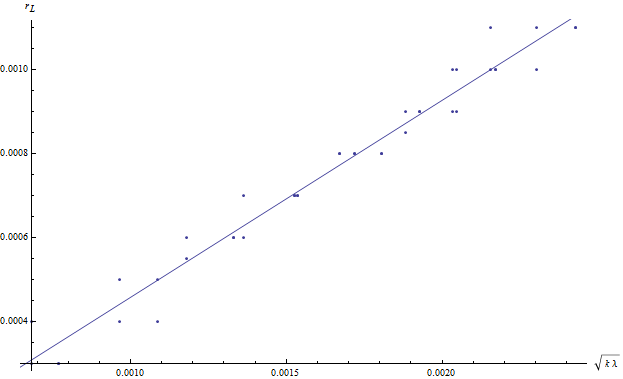
\includegraphics[width=0.8\textwidth]{bilder/aufgabe11.png}\\
	\end{tabular}
	\caption{Punkte und lineare Regressionsgerade zur Krümmungsradiusbestimmung $R$}
	\label{fig:aufgabe11}
\end{figure}
Die in Abbildung \ref{fig:aufgabe11} eingezeichnete Gerade erfüllt die Gleichung:
\begin{equation*}
y=0.468428x-0.0000105591
\end{equation*}
Somit beträgt der Krümmungsradius $R=\unit[0.47]{m}$.
\subsection{Bestimmung des Brechungsindizes von Wasser}
In diesem Versuch sollten wir das Brechungsindex von Wasser bestimmen, indem wir die gleiche Messungen wie in Aufgabe 1.1 durchführen, mit dem Unterschied dass zwischen Linse und Objektträger statt Luft sich Wasser befindet. Dazu brachten wir einige Tropfen Wasser dazwischen.\\ \\
Dieses Mal war das Bild der newtonschen Ringe verschwommen, die Übergänge hell zu dunkel waren dabei sehr schwer zu erkennen. Deshalb konnten wir an der rechten Seite vom Mittelpunkt der Ringe bis zu 5 und an der linken bis zu 8 Ringe messen.\\
Wir können zur Brechungsindexbestimmung die Messdaten aus Aufgabe 1.1 für die Luft wiederverwenden und das Brechungsindex einfach anhand unterer Formel bestimmen (s. Vorbereitung):
\begin{equation*}
n_W=\frac{r_L^2}{r_W^2} \cdot n_L \quad \text{wegen} \quad n_L \approx 1 \Rightarrow \quad n_W=\frac{r_L^2}{r_W^2}
\end{equation*}
Es ist wieder die Bestimmung einer Regressiongerade notwendig, indem man man $r_L^2$ über $r_W^2$ aufträgt:
\begin{equation*}
r_L^2=n_W\cdot r_W^2
\end{equation*}
Die aus unseren Messwerten bestimmte Regressionsgerade lautet:
\begin{equation*}
n_W=1.06684x + 4.07808 \cdot 10^{-9}
\end{equation*}
Wir erhalten das Brechungsindex des Wassers mit $n_W=1.07$, welches vom Literaturwert $n_{W,lit}=1.33$ um $\unit[29.73]{\%}$ abweicht.
\subsection{Bestimmung der Brennweite der Linse durch Autokollimation}
Es musste die Brennweite der Linse mittels Autokollimation bestimmt werden. Dazu stellten wir eine Linse vor einem Spiegel und vor der Linse ein selbstleuchtender Gegenstand. Dabei variierten wir den Abstand selbstleuchtender Gegenstand-Linse bis der Schatten des Gegenstandes auf sich selbst scharf und seitenverkehrt abgebildet wurde.\\ \\
Dabei entsprach der Abstand Gegenstand-Linse der gesuchten Brennweite $f$. Wir haben die Positionen des Gegenstands gemessen, bei denen der Schatten den o.g. Kriterien entsprach.
\begin{table}[H]
\begin{tabular}{c|c|c}
	Position Linse $(cm)$ & Position Gegenstand $(cm)$ & Brennweite $(cm$) \\
	\hline
	35.2 & 15.95 & 19.25 \\
	35.2 & 15.9 & 19.3 \\
	35.2 & 15.7 & 19.5 \\
	35.2 & 15.5 & 19.7 \\
\end{tabular}
\caption{Positionen der Linse und des Gegenstands, bei denen ein scharfes, seitenverkehrtes Schatten entstand}
\label{tab:aufgabe13}
\end{table}
Aus den obigen Brennweiten, bestimmten wir als Brennweite der Linse deren Mittelwert mit $\overline{f}=\unit[19.44]{cm}$. Diese Brennweite stimmt somit mit denen der im Labor vorhanden Linsen, die Brennweiten zwischen $\unit[5]{cm}$ und $\unit[35]{cm}$ aufwiesen.
\begin{figure}[H]
	\centering
	\begin{tabular}{@{}r@{}}
		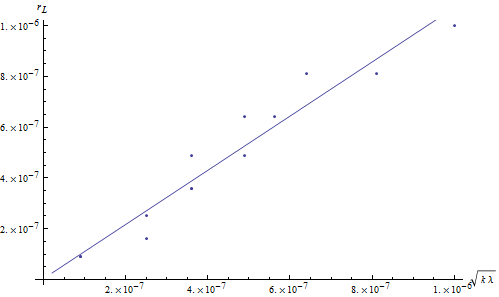
\includegraphics[width=0.6\textwidth]{bilder/aufgabe12.png}\\
	\end{tabular}
	\caption{Punkte und lineare Regressionsgerade zur Bestimmung des Brechungindizes des Wassers}
	\label{fig:aufgabe12}
\end{figure}
\subsection{Bestimmung der Brechungsindex des Linsenglases aus $R$ und $f$}
Es sollte nun das Brechungsindex des Linsenglases aus den zuvor bestimmten Krümmungsradius $R$ und Brennweite $f$ ermittelt werden. Wir nutzen die in der Vorbereitung bewiesene Formel:
\begin{equation*}
R=2(n-1)f \quad \Rightarrow \quad n=\frac{R}{2f}+1=\frac{\unit[0.47]{m}}{2 \cdot \unit[0.19]{m}}+1=2.24
\end{equation*}
Glase habe Brechungsindizes zwischen 1.45 und 2.14 \cite{wiki:brechungsindex}. Damit liegt unser Wert ausserhalb dieses Bereiches, was vielleicht daran liegt, dass der Wert, den wir in Aufgabe 1.1 für den Krümmungsradius $R$ bestimmt haben, nicht so genau war.
\section{Beugung am Gitter}
\subsection{Justieren des Gitterspektrometers}
\subsection{Bestimmung der Gitterkonstante}
\subsection{Wellenlängenabstand der gelben Na-Linien}
\subsection{Bestimmung der Gitterkonstanten eines unbekannten Gitters}

\newpage

\bibliographystyle{plain}
\bibliography{quellen}

\end{document}